\documentclass{ip-doc}

\title{Example IP Module}
\author{Wuqiong Zhao}
\version{1.0}

\begin{document}
\maketitle

\section{Introduction}
\begin{factstable}
\rowcolors{2}{gray!10}{white}
\renewcommand{\arraystretch}{1.2}
\begin{tabularx}{\linewidth}{l|X}
\toprule
  Name & Example IP \\
  Identifier & \texttt{org.wqzhao.example\_ip} \\
  Version & \theversion \\
  Author & \href{https://wqzhao.org}{Wuqiong Zhao} {\scriptsize(me@wqzhao.org)} \\
  Device & AMD UltraScale+ \\
  Platform & Vivado \\
  Design Files & Verilog \\
  Simulation Model & Verilog \\
  Constraints File & N/A \\
\bottomrule
\end{tabularx}
\end{factstable}

The ``Example IP'' is just an example.
You will need to create your own IP module to use this class to document it elegantly.
This \texttt{ip-doc} class is designed to help you write beautiful documentation for your IP modules,
so you can concentrate on contents only.
Basic \LaTeX{} knowledge is required to use this class.
Yet, you may further customize this class to suit your needs.

I have been working with RFSoC for a while,
and I found that the documentation for IP modules is often not as good as it should be.
Therefore, I created this class to make it easier for me to document my custom IP modules.
I hope you find it useful too.

This \LaTeX{} class is maintained by
\href{https://github.com/Teddy-van-Jerry}{Teddy van Jerry}
(\href{https://wqzhao.org}{Wuqiong Zhao}).

\section{Features}
This module is only an example with minimal features.
The features of this IP module are:

\begin{itemize}
  \item Support AXI4 interface.
  \item Some features related to \LaTeX{} which is unfortunately not hardware.
  \begin{itemize}
    \item Beautiful documentation for you to concentrate on writing good contents.
    \item Easy to use and customize thanks to the LaTeX3 technology.
    \item Fully open source and free at \url{https://github.com/Teddy-van-Jerry/ip-doc}.
  \end{itemize}
  \item Other features that you want to impress your users.
\end{itemize}

\section{Usage}

\subsection{Fundamentals}
This class can be used with any \LaTeX{} engine,
including \texttt{pdflatex}, \texttt{lualatex}, and \texttt{xelatex}.

\subsection{Text}
The text is in sans-serif font ``TeX Gyre Heros,'' a ``Helvetica'' clone.
Section numbers are in the left margin.

\subsubsection{Subsubsection}
Here is a subsubsection, the smallest sectioning command that comes with numbering.

\paragraph{Paragraph.}
Here is a paragraph, which has a run-in header.

\subsection{Math}
Math fonts are still the serif ones.
For example $a^2 + b^2 = c^2$.
Display equations can also be used:
\begin{equation}
  \int_0^1 x^2 \, \mathrm{d}x = \frac13.
\end{equation}

\subsection{Figures and Tables}
Figures and tables are useful to illustrate your IP module.
Figure~\ref{fig:example} shows a waveform plot of integrated logic analyzer (ILA) captured QPSK packet.
\begin{figure}[htbp]
  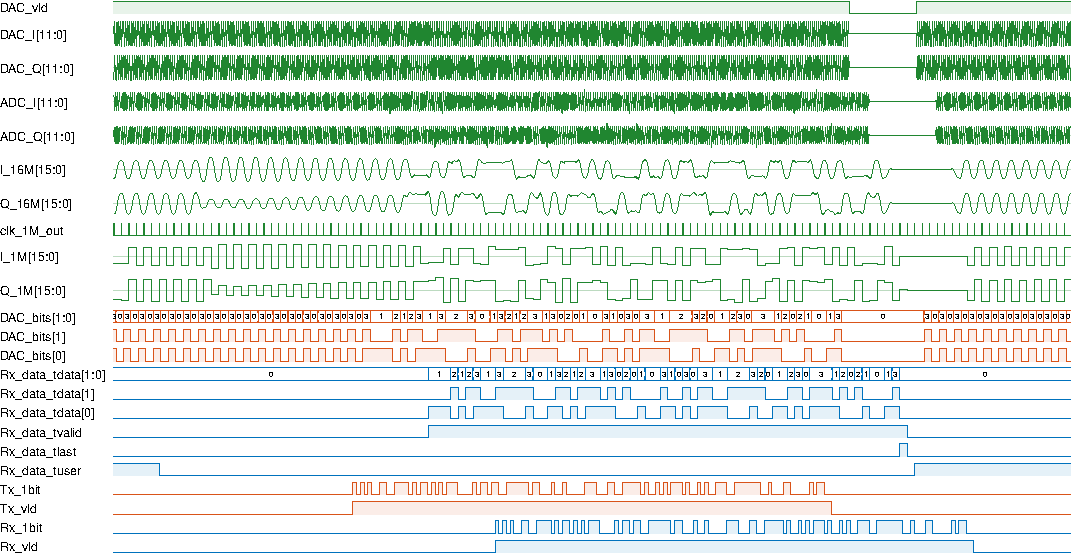
\includegraphics[width=\linewidth]{fig/ila_QPSK-crop.pdf}
  \caption{A QPSK packet captured by ILA. \cite{zhao2024dual}}
  \label{fig:example}
\end{figure}

\section{Know Issues}
\begin{enumerate}
  \item The \texttt{factstable} environment internally uses the \texttt{wrapstuff} package, which may cause some issues.
  Its position may not be as expected, so you may add parameters to the \texttt{wrapstuff} environment via the first optional argument of the \texttt{factstable} environment.
  Another known issue is in some places the \texttt{itemize} and \texttt{enumerate} environment has to be separated by a blank line (or {\ttfamily\string\par\relax}) from the text.
  \item The documentation of this class is not complete.
\end{enumerate}

\section{Further Readings}
Ti\textit{k}Z is useful to create beautiful diagrams in \LaTeX.
These can be useful to illustrate the architecture of your IP module.
An example paper about high-level-synthesis (HLS) using Ti\textit{k}Z is \cite{zhao2024flexible},
with open access PDF at \url{https://wqzhao.org/assets/zhao2024flexible.pdf}.

% comment out if you do not have a bibliography file
\bibliographystyle{plain}
{\small\bibliography{ip-doc-example}}

\end{document}
